\documentclass[11pt,a4paper]{article}
\usepackage[utf8]{inputenc}
\usepackage[T1]{fontenc}
\usepackage[francais]{babel}
%\usepackage{fullpage}
\usepackage{gensymb}
\usepackage{graphicx}
\usepackage{float}
\usepackage{amsmath}
\usepackage{listings}
\usepackage{etoolbox}
\usepackage[tocindentauto]{tocstyle}
\usetocstyle{KOMAlike}


\usepackage{hyperref}
\hypersetup{
    colorlinks,
    citecolor=black,
    filecolor=black,
    linkcolor=black,
    urlcolor=black
}

\renewcommand\thesection{\Roman{section}}
\renewcommand\thesubsection{\arabic{subsection}.}
\renewcommand\thesubsubsection{\alph{subsubsection}.}

\preto{\section}{\clearpage}

\title{Étude et réalisation d'une chaîne de streaming vidéo}
\author{Raffi Tchoboian \& Simon Le Guével}

\begin{document}

\pagenumbering{gobble}
\maketitle

\vspace{1cm}
\begin{center}
Rapport de PFE
\\
Département Télécommunications, Services \& Usages
\end{center}

\vspace{3.5cm}

\noindent
Tuteurs :

Khalid IDRISSI, Maître de conférences à l'INSA de Lyon

Philippe ISORCE, Professeur associé à l'INSA de Lyon

\vspace{5cm}
\begin{center}
\includegraphics[scale=0.5]{images/insa.png}
\end{center}

\newpage

\section*{Remerciements}

Nous remercions nos tuteurs, Khalid IDRISSI et Philippe ISORCE, pour leur aide quant à la mise en place du sujet et à leur suivi sans faille tout au long du projet.
Nous remercions aussi Razvan STANICA pour sa supervision des PFE ainsi que Julien PONGE et Frédéric LE MOUËL pour l'évaluation de la soutenance orale.
Merci aussi au jury chargé d'évaluer ce présent rapport.

\bigbreak
Enfin, un grand merci à l'équipe du département Télécommunications de l'INSA de Lyon pour les enseignements transmis et le matériel mis à notre disposition.

\newpage

\setcounter{tocdepth}{2}
\tableofcontents

\newpage
\pagenumbering{arabic}

\section{Présentation du projet}

\subsection{Objectif général}
L'objectif général de notre projet de fin d'études, dit \textit{PFE}, est d'étudier et de mettre en place une chaîne de transmission vidéo.
Nous ferons l'étude technique et la réalisation de l'ensemble des étapes : de la station émettrice au récepteur, en passant par les techniques de mise en réseau.
Notre projet servira alors de base dans le cadre de travaux pratiques de la formation Télécom à l'INSA de Lyon.

\bigbreak
Nous avons décidé de nous intéresser plus particulièrement à l'amélioration de la qualité d'une zone géographique d'un flux vidéo, au détriment du reste de la vidéo.

Ce principe peut se révéler intéressant dans des cas où le consommateur d'un flux vidéo ne serait intéressé que par une zone précise d'une image capturée par une caméra, tout en étant susceptible de changer de zone d'intérêt à tout instant.
La zone d'intérêt est choisie et commandée par le client récepteur du flux vidéo, afin que l'émetteur puisse adapter la zone d’intérêt pour la suite de la transmission.

\bigbreak
Nous essaierons de faire des choix technologiques les plus simples et compréhensibles possibles et d'assurer une interopérabilité entre différentes plateformes matérielles et logicielles.

\subsection{Cas d'application}

Afin d'illustrer ce système en pratique, nous l'implémenterons au sein d'une solution de transmission vidéo distante en réalité virtuelle.
Une station émettrice mobile capture un flux vidéo provenant d'une caméra à grand angle et transmet un flux qui sera alors reçu sur un autre terminal mobile n'affichant qu'une zone précise de l'image à travers une solution de réalité virtuelle de type Google Cardboard.
Le terminal est donc déplacé avec les mouvements de tête du spectateur et la zone de visionnage est donc déplacée en conséquence pour obtenir un effet immersif.
La nouvelle zone d’intérêt est renvoyée du terminal mobile à l'émetteur pour faire à nouveau coïncider la zone visionnée avec la région d'intérêt à qualité améliorée.

\bigbreak
Nous implémenterons aussi un récepteur sur ordinateur afin de montrer l'interopérabilité de notre solution.
Ce récepteur aura disposera aussi des fonctionnalités de déplacement de la zone d'intérêt.

\subsection{Contraintes qualitatives}

Nous avons la contrainte de transmettre l’ensemble de la vidéo pour pouvoir répondre instantanément aux déplacements de la tête de spectateur.
En effet, des solutions existantes comme celle choisie par certains drones tels que celui de Parrot font le choix de ne transmettre que la région d’intérêt. Cela présente l’inconvénient de devoir attendre un aller/retour complet de transmission avant d’avoir l’image demandée. Pour un effet immersif complet, cela ne peut pas être envisagé.
D’autres solutions font le choix de simplement transmettre l’image complète non-modifiée, assurant ainsi une image de qualité moyenne sur l’ensemble de la scène.

\bigbreak
Notre solution devra donc permettre d’avoir une qualité supérieure de la zone observée au prix d’une dégradation du reste de l’image.
Ainsi, lorsque le spectateur bouge la tête, il voit immédiatement la partie de l’image correspondante, mais en qualité dégradée. Il faudra attendre l’aller/retour complet pour obtenir une image de bonne qualité.

\bigbreak
Pour pouvoir mesurer une amélioration de la qualité et s’adapter à diverses conditions de transmissions réseau, nous utiliserons un encodeur à débit contraint, de telle sorte que ce soit la qualité qui soit variable.
Ce débit pourra d’ailleurs être adapté en fonction des pertes réseaux observées par le récepteur.


\section{Recherche}

Nous avons sélectionné quelques papiers qui s'intéressent à des techniques s'approchant de notre projet : la compression vidéo avec une qualité variable en fonction de la zone d'intérêt de l'utilisateur.

\bigbreak
La solution la plus évidente est d'intervenir directement au niveau de l'algorithme de compression.
L'article de Amir Said et William Pearlman [1] décrit comment compresser une image avec un débit variable pour chaque partie de l'image.

Cette approche est intéressante mais nous faisons le choix de réutiliser un algorithme de compression, dit \textit{codec}, existant.
L'algorithme étant notamment déjà intégré dans les terminaux de réception pour effectuer du décodage matériel, il nous est presque impossible d'intervenir à ce niveau.

\bigbreak
L'article de Engin Kurutepe [2] montre comment optimiser l'envoi d'un flux provenant de plusieurs caméras.
Pour cela, l'équipement récepteur suit les mouvements de la tête de l'utilisateur afin de savoir quelle zone de l'image l'intéresse le plus.
Après cela, l'équipement envoie cette information à l'encodageur qui va demander un plus gros débit aux caméras qui filment la zone d'intérêt et un débit plus faible aux autres caméras.

Nous ne pouvons pas réutiliser ce concept car nous n'avons qu'une seule caméra qui filme la scène et le principe décrit par l'article est applicable seulement pour une même scène filmée avec plusieurs caméras.
Cela nous a tout de même confortés dans l'idée d'encoder une vidéo sphérique avec une qualité dynamique, mais à l'intérieur d'une même image.

\bigbreak
	Enfin, l'article de Aditya Mavlankar et Bernd Girod [3] explique comment optimiser l’envoi d’une image basse qualité d’un match de football ainsi qu’une zone précise de haute qualité.
L’idée ressemble à ce que nous voulons faire, mais les recherches se portent sur l’optimisation de l’encodage pour du broadcast ; comment éviter d’encoder le flux de haute qualité pour chaque téléspectateur.
Or, notre projet fonctionne dans un modèle mono-utilisateur, il sera donc plus simple et plus efficace pour notre modèle d’encoder le flux entier en prenant directement en compte la zone d'intérêt de l'utilisateur.
Aussi, cet article cite les mécanismes FMO et ASO du standard de compression vidéo H.264 qui permettent respectivement d’avoir un débit différent pour chaque bloc de l'image et de prioriser la qualité des zones de l’image.
Malheureusement, ces plugins ne sont pas implémentés par défaut dans des outils libres comme FFmpeg ou la libx264 et peu de récepteurs mobiles ne les comprennent.

\bigbreak
Globalement, nous n'avons pas pu trouver d'articles décrivant un procédé permettant d'implémenter directement notre projet, nous partirons donc sur l'étude et la conception d'une solution propre.
Cette recherche nous aura tout de même permis d'avoir un bon aperçu des techniques de compression vidéo couramment utilisées.


\section{Architecture générale}
Notre solution s'articule autour d'un émetteur (un Raspberry Pi 3) et de deux récepteurs (un smartphone Android et un ordinateur sous Linux).
Pour rappel, notre objectif n'est pas de tout réimplementer mais d'utiliser des briques logicielles dédiées au streaming vidéo.

\subsection{Canaux de communications}
L'émetteur et le récepteur communiquent via un réseau Wi-Fi créé à partir d'un routeur tierce.
Il y a deux sockets qui relient les deux équipements :

\bigbreak
\begin{itemize}
\item{Socket \texttt{UDP} : le flux vidéo envoyé depuis l'émetteur vers le récepteur}
\item{Socket \texttt{TCP} : le canal de contrôle qui permet au récepteur de déplacer la zone d'intérêt}
\end{itemize}

\subsection{L'émetteur}
L'émetteur est un Raspberry Pi 3 sur lequel est connecté une caméra grand angle.
Pour récupérer le flux RAW de la caméra, nous utilisons une première instance de \texttt{FFmpeg} (un logiciel open-source dédié au traitement des images et vidéos).
Ce flux RAW est redirigé vers notre programme, écrit en C, qui va se charger de traiter le flux vidéo en détériorant les parties de l'image qui n'intéressent pas l'utilisateur.
Ce flux traité est dirigé vers une deuxième instance de \texttt{FFmpeg}, qui va encoder le flux RAW en un flux H.264 et l'envoyer en \texttt{UDP} au récepteur.
Par ailleurs, c'est le programme écrit en C qui fait office de serveur \texttt{TCP} afin de recevoir les demandes de déplacement de la zone d'intérêt.

\bigbreak
\begin{figure}[H]
\begin{center}
\includegraphics[scale=0.35]{images/schema_emetteur.png}
\end{center}
\caption{Schéma de l'émetteur}
\label{}
\end{figure}
\bigbreak

\subsection{Récepteur Android}
Notre premier récepteur est une application Android fonctionnant dans un smartphone qui se trouve dans un casque de réalité virtuelle.
L'application commence par récupérer le flux \texttt{UDP} d'où elle extrait le flux vidéo H.264.
Ce flux est décompréssé par le décodeur interne d'Android.
Le flux décodé est alors traité par notre application pour lui redonner son aspect initial, puis il est redirigé vers une surface pour être affiché à l'écran.
Par ailleurs, l'application possède un client TCP pour se connecter au canal de contrôle de l'émetteur.

\bigbreak
\begin{figure}[H]
\begin{center}
\includegraphics[scale=0.35]{images/schema_recepteur_android.png}
\end{center}
\caption{Schéma du récepteur Android}
\label{}
\end{figure}

\bigbreak
Cette application est aussi responsable de la gestion de la réalité virtuelle de notre projet : elle gère les déplacements de la tête de l'utilisateur et adapte la zone vidéo observée en conséquence.

\subsection{Récepteur ordinateur}
Nous deuxième récepteur fonctionne sur un ordinateur sous Linux. Il affiche la vidéo grand angle et permet de déplacer (via le clavier) la zone d'intérêt.
Pour fonctionner, il récupère le flux H.264 via une instance de \texttt{FFmpeg} qui décompresse la vidéo.
Le flux RAW est redirigé vers notre programme écrit en C qui traite la vidéo, afin de lui redonner son aspect initial, et l'affiche dans une fenêtre.
De plus, le programme possède un client \texttt{TCP} pour le canal de contrôle.

\bigbreak
\begin{figure}[H]
\begin{center}
\includegraphics[scale=0.35]{images/schema_recepteur_linux.png}
\end{center}
\caption{Schéma du récepteur Android}
\label{}
\end{figure}

\bigbreak
Dans la partie suivante de ce rapport, nous détaillerons et motiverons les choix techniques réalisés pour l'ensemble de ces briques logicielles.

\section{Détails d'implémentation}

\subsection{Acquisition d'image RAW}
Pour notre projet, nous nous sommes procuré une caméra à grand angle (180\degree) pour être en mesure de filmer l'intégralité d'une scène.

\bigbreak
La caméra est compatible avec le driver générique \texttt{uvcvideo} inclus par défaut dans le noyau Linux, et peut donc être utilisée à travers \textit{Video4Linux 2}, V4L2.

\bigbreak
Afin d'obtenir l'image la moins altérée possible et de faciliter les futurs traitements sur l'image, nous récupérons les images RAW non-compressées.
La caméra est capable, à travers l'USB2, de tenir un flux de données correspondant à des images d'une résolution de \texttt{1280x720} à une fréquence de 10 images par seconde.
% Détail sur le débit en sortie du port USB ?

\bigbreak
L'acquisition est réalisée grâce à notre première instance de \texttt{FFmpeg} et à son module d'acquisition V4L2 qui permettent d'obtenir les octets correspondants sur la sortie standard pour la suite de notre traitement.

\bigbreak
La caméra utilisée présente une particularité : le capteur CMOS utilisé est un capteur standard et l'effet grand angle est obtenu par l'apposition d'une lentille convexe au-dessus.
Si cela permet alors d'obtenir un champ de vision très proche de 180\degree, l'image en retour présente un effet \textit{fisheye} non-négligeable.

\bigbreak
\begin{figure}[H]
\begin{center}
\includegraphics[scale=0.2]{images/fisheye.png}
\end{center}
\caption{Effet fisheye induit par la lentille}
\label{}
\end{figure}
\bigbreak

Pour rendre des proportions réalistes aux abords de l'image, il est nécessaire de procéder à une correction de la déformation induite par la lentille.
Heureusement, \texttt{FFmpeg} dispose d'un certain nombre de plugins de traitement d'image que nous pouvons utiliser pendant la phase d'acquisition d'image RAW.

\bigbreak
L'un d'entre eux, issu de la collection de plugins \texttt{Frei0r}, est le plugin \texttt{Defish0r}, relativement simple d'utilisation et qui permet d'annuler cet effet de distorsion.
Malheureusement, les premiers tests ont montré que le plugin était trop gourmand en calcul CPU, et qu'il était impossible de traiter 10 images par seconde : le retard s'accumule rapidement.

\bigbreak
Un autre plugin, plus générique, est présent dans \texttt{FFmpeg} : \texttt{lenscorrection}.
Plus léger en calcul, il est capable de traiter nos 10 images par seconde avec notre carte Raspberry Pi 3.
Son inconvénient est son paramétrage : le filtre demande deux coefficients correspondant aux termes de second et quatrième degrés dans la formule de correction :

$$r_{src} = r_{targ} * (1 + k1*(\frac{r_{targ}}{r_0})^2 + k2*(\frac{r_{targ}}{r_0})^4)$$
avec :
\begin{itemize}
\item{$k1$, $k2$ : coefficients considérés}
\item{$r_0$ : moitié de la diagonale de l'image}
\item{$r_{src}$ : distance entre le point considéré dans l'image source et le centre de l'image}
\item{$r_{targ}$ : distance du point à placer dans l'image de destination avec le centre de l'image}
\end{itemize}

\bigbreak

La difficulté réside donc dans la détermination des coefficients $k1$ et $k2$ adaptés à notre ensemble \{capteur+lentille\}.
Les valeurs se situant dans l'intervalle $[-1;1]$, nous réalisons un test visuel en générant des images avec tous les couples de $(k1, k2)$ possibles en prenant un pas de $p=0.1$, soit une série de 441 images.

\bigbreak
\bigbreak
\begin{figure}[H]
\begin{center}
\includegraphics[scale=0.3]{images/fisheye_tries.png}
\end{center}
\caption{Essais de coefficients de correction}
\label{}
\end{figure}
\bigbreak

\bigbreak
Le détermination des coefficients s'est donc faite de façon qualitative en visionnant la série d'images et en choisissant l'image présentant le moins de déformation tout en évitant les aberrations.
Les valeurs suivantes semblent correspondre à notre lentille :
$$k1 = -0.4, k2 = 0.1$$

\subsection{Traitement de l'image YUV}
Si nous avons maintenant une image brute corrigée, nous souhaitons lui appliquer notre traitement spécifique.

\subsubsection{Format \texttt{YUV 4:2:0}}
L'image RAW d'entrée est donc d'une résolution de \texttt{1280x720} pixels avec un codage des pixels selon le format \texttt{YUV 4:2:0}.
Ce format est très utilisé dans le codage de la vidéo car il est adapté à un visionnage par un œil humain : contrairement au format \texttt{RGB} qui code de façon égale les composantes rouge, verte et bleue de la vidéo, le format \texttt{YUV} code une information de luminance et une information de chrominance.
Dans le cas du format \texttt{YUV 4:2:0}, il y a deux fois plus d'informations de luminance que de chrominance, tout simplement car l'œil humain est plus sensible aux différences de luminosité qu'aux différences de teinte.

\bigbreak
Plus précisément, les pixels sont répartis en blocs de 4 pixels (\texttt{2x2}).
Chaque bloc contient 4 informations de luminance (une valeur \texttt{Y} pour chacun des 4 pixels), mais seulement une information de chrominance commune à l'ensemble du bloc (une valeur \texttt{U} et une valeur \texttt{V}).

\begin{figure}[H]
\begin{center}
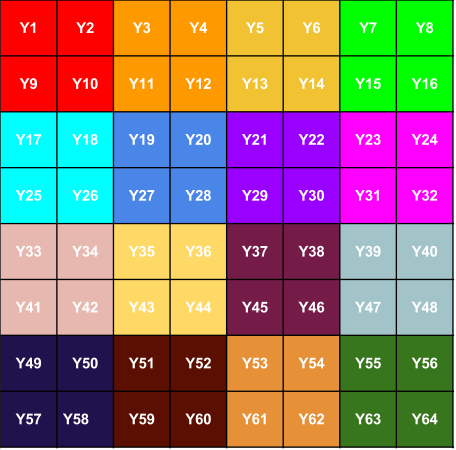
\includegraphics[scale=0.5]{images/yuv1.png}
\end{center}
\caption{Organisation des pixels au sein d'une image \texttt{YUV 4:2:0}}
\label{}
\end{figure}

\bigbreak
Chaque valeur de \texttt{Y}, \texttt{U} et \texttt{V} est codée sur un octet.
Ainsi, la taille d'une image \texttt{YUV} d'une résolution de \texttt{8x8} pixels (16 blocs) comme celle ci-dessus peut être calculée comme ceci :

$$ T = 16 * (4Y + 1U + 1V) = \mathbf{96}$$

\bigbreak

D'une manière générale, la taille d'une image \texttt{YUV 4:2:0} peut donc se calculer comme étant le nombre de pixels multiplié par $\frac{3}{2}$.
Ainsi, chacune de nos images \texttt{1280x720} a une taille d'environ 1,4 Mo.

\bigbreak
La répartition de ces informations dans la suite d'octets est un peu particulière : on trouve d'abord toutes les valeurs \texttt{Y}, puis toutes les valeurs \texttt{U} et enfin \texttt{V}.
La lecture d'un bloc se fait donc en trois lectures successives.

\begin{figure}[H]
\begin{center}
\includegraphics[scale=0.5]{images/yuv2.png}
\end{center}
\caption{Séquence d'information du format \texttt{YUV 4:2:0}}
\label{}
\end{figure}

\bigbreak

\subsubsection{Traitement spécifique}

Puisque nous avons fait le choix de ne pas intervenir au niveau du codec lui-même, nous appliquons un traitement spécifique permettant de sous-échantillonner les zones autres que la zone d'intérêt.
L'idée est de conserver la zone d'intérêt dans sa résolution originelle et de diviser par un facteur quatre les dimensions des autres parties de l'image, c'est-à-dire diviser la largeur et la hauteur par deux.

\bigbreak
La zone d'intérêt a une dimension fixe choisie comme une moitié de largeur et hauteur totales, soit une résolution de \texttt{640x360} pixels ou $\frac{1}{4}$ de la surface de l'image source.
Ainsi, dans l'idéal, notre image traîtée finale a une résolution d'une fraction de celle de l'image source :

$$ R = \frac{1}{4} + \frac{3}{4}*\frac{1}{4} = \mathbf{\frac{7}{16}} $$

\bigbreak

Ce résultat est celui que nous pourrions obtenir en découpant de façon idéale les zones.
Pour des raisons de complexité de calculs, nous essaierons de garder les zones entières lors de nos déplacements.

\begin{figure}[H]
\begin{center}
\includegraphics[scale=0.4]{images/decoupage.png}
\end{center}
\caption{Découpage en zones d'une image 16:9}
\label{}
\end{figure}

\bigbreak
La zone d'intérêt, ou ZOI, conserve ses dimensions d'origine : \texttt{640x360}.
Elle est placée dans la seconde moitié de l'image, laissant ainsi une autre fenêtre de \texttt{640x360} pixels libre.

\bigbreak
Pour rappel, la ZOI a une taille fixe mais sa position de départ est variable et contrôlée par le client récepteur.
Ainsi, les autres zones autour de cette ZOI sont de taille variable, en fonction du point de départ de la ZOI que nous définirons par le couple \texttt{(zoiX, zoiY)}.
Les positions et dimensions des différentes zones sont alors définies comme cela :
\bigbreak
\begin{itemize}
\item{Zone 1 : position=\texttt{(0, 0)} ; dimensions=\texttt{(zoiX, imgHeight)}}
\item{Zone 2 : position=\texttt{(zoiX+zoiW, 0)} ; dimensions=\texttt{(imgWidth-(zoiX+zoiW), 720)}}
\item{Zone 3 : position=\texttt{(zoiX, 0)} ; dimensions=\texttt{(zoiW, zoiY)}}
\item{Zone 4 : position=\texttt{(zoiX, zoiY+zoiH)} ; dimensions=\texttt{(zoiW, imgHeight-(zoiY+zoiH))}}
\end{itemize}

\bigbreak
avec :
\begin{itemize}
\item{\texttt{(zoiX, zoiY)} : position actuelle de la ZOI}
\item{\texttt{(zoiW, zoiH)} : taille de la ZOI, dans notre cas \texttt{(640, 360)}}
\item{\texttt{(imgWidth, imgHeight)} : dimensions de l'image d'origine, dans notre cas \texttt{(1280, 720)}}
\end{itemize}

\bigbreak
Les quatre zones sont ensuite sous-échantillonnées : les largeurs et hauteurs sont divisées par deux, procédant ainsi à une réduction de la résolution d'un facteur 4.
Pour cela, nous transformons chaque groupe de quatre blocs \texttt{YUV} en un seul bloc selon le procédé suivant :

\begin{figure}[H]
\begin{center}
\includegraphics[scale=0.5]{images/yuv3.png}
\end{center}
\caption{Approximation des blocs}
\label{}
\end{figure}

\bigbreak

Chaque bloc réduit est donc l'approximation des quatre blocs qu'il contient.
Pour rappel, un bloc est composé de quatre pixels et contient une information de luminance pour chacun des pixels, mais une seule information de chrominance pour l'ensemble du bloc.
Le bloc réduit est donc constitué d'une seule information de chrominance comme étant la moyenne des chrominances des quatre blocs d'origine ; et de quatre informations de luminance, chacune étant la moyenne des luminances de chaque blocs.

\bigbreak
Par exemple, pour le premier bloc réduit, le calcul est fait comme ceci :
\medbreak
$Y_{reduit}[0] = \frac{Y1 + Y2 + Y9 + Y10}{4}$
\medbreak
$Y_{reduit}[1] = \frac{Y3 + Y4 + Y11 + Y12}{4}$
\medbreak
$Y_{reduit}[2] = \frac{Y17 + Y18 + Y25 + Y26}{4}$
\medbreak
$Y_{reduit}[3] = \frac{Y19 + Y20 + Y27 + Y28}{4}$
\medbreak
$U_{reduit} = \frac{U1 + U2 + U5 + U6}{4}$
\medbreak
$V_{reduit} = \frac{V1 + V2 + V5 + V6}{4}$

\bigbreak


\begin{figure}[H]
\begin{center}
\includegraphics[scale=0.5]{images/yuv4.png}
\end{center}
\caption{Blocs réduits}
\label{}
\end{figure}

\bigbreak
Après avoir appliqué cette transformation sur l'ensemble de nos quatre blocs, on obtient quatre blocs aux dimensions variables en fonction de \texttt{zoiX} et \texttt{zoiY}.
Il existe cependant différents agencements possibles de nos blocs qui donnent des dimensions constantes.
Après avoir réduit nos zones selon le principe que l'on vient de décrire, on leur trouve les dimensions suivantes :

\bigbreak
\begin{itemize}
\item{Zone 1 : \texttt{($\frac{\text{zoiX}}{2}$, $\frac{\text{imgHeight}}{2}$)}}
\item{Zone 2 : \texttt{($\frac{\text{imgWidth}-(\text{zoiX}+\text{zoiW})}{2}$, $\frac{\text{imgHeight}}{2}$)}}
\item{Zone 3 : \texttt{($\frac{\text{zoiW}}{2}$, $\frac{\text{zoiY}}{2}$)}}
\item{Zone 4 : \texttt{($\frac{\text{zoiW}}{2}$, $\frac{\text{imgHeight}-(\text{zoiY}+\text{zoiH})}{2}$)}}
\end{itemize}

\bigbreak
On peut tout de suite trouver un assemblage constant pour les zones 1 et 2 réduites : elles font la même hauteur et leur largeur commune ne dépend pas de la position de la ZOI : elles sont complémentaires.

$$ W_1 + W_2 = \frac{zoiX}{2} + \frac{imgWidth-(zoiX+zoiW)}{2} = \frac{imgWidth - zoiW}{2}$$
$$ = \mathbf{\frac{imgWidth}{4}} $$

\bigbreak
Les zones 1 et 2 l'une à côté de l'autre forment donc une zone de dimension constante \texttt{($\frac{imgWidth}{4}$, $\frac{imgHeight}{2}$)}.
Le même principe s'applique aux zones 3 et 4, avec cette fois-ci une largeur constante :

$$ H_3 + H_4 = \frac{zoiY}{2} + \frac{imgHeight-(zoiY+zoiH)}{2} = \frac{imgHeight - zoiH}{2} $$
$$ = \mathbf{\frac{imgHeight}{4}} $$

\bigbreak
Les zones 3 et 4 l'une après l'autre forment donc une zone de dimension constante \texttt{($\frac{imgWidth}{4}$, $\frac{imgHeight}{4}$)}.
Nous avons choisi d'utiliser la répartition suivante :

\begin{figure}[H]
\begin{center}
\includegraphics[scale=0.4]{images/decoupage2.png}
\end{center}
\caption{Organisation des zones}
\label{}
\end{figure}

\bigbreak
Nous obtenons ainsi une image d'une résolution de \texttt{640x720} pixels contenant notre ZOI inchangée et les autres zones sous-échantillonnées.
L'image après notre traitement ne pèse donc plus que la moitié de sa taille d'origine, avec un petit écart par rapport aux $\frac{7}{16}$ théoriques calculés.
Cet écart correspond à la zone verte sur notre schéma et ne véhicule aucune information vidéo.
Nous pourrions arranger différement les blocs en les découpant davantage mais nous avons fait le choix de conserver des blocs entiers pour éviter un calcul supplémentaire côté récepteur.

\subsection{Compression vidéo et transmission}
Une fois notre image modifiée, l'étape suivante est de la compresser et de la transmettre au périphérique récepteur.

\subsubsection{Initialisation réseau}
Notre programme principal, que l'on nommera \textit{handler} dans la suite de ce rapport, gère le flux RAW d'entrée, la connexion avec le récepteur, et l'interaction avec notre compresseur vidéo.
Au lancement du programme, le programme crée une socket d'écoute \texttt{TCP} sur le port \texttt{1234}.
C'est sur ce port que le client récepteur doit venir initier une connexion.

\bigbreak
À la première connexion détectée et une fois le \textit{handshake} \texttt{TCP} effectué, notre programme connaît alors l'adresse IP du récepteur intéressé par notre flux vidéo.
Cette socket \texttt{TCP} restera ouverte entre l'émetteur et le récepteur pour la signalisation par la suite.

\subsubsection{Envoi des images vidéo}
Notre programme se met à lire son entrée standard sur laquelle sont envoyées les images RAW de la caméra (par la première instance \texttt{FFmpeg}) puis lui applique notre traitement spécifique.
Il lance ensuite une seconde instance de \texttt{FFmpeg}, configurée cette fois-ci en tant qu'encodeur vidéo.
L'instance prend en entrée nos images RAW traitées d'une résolution de \texttt{640x720} et les encode en utilisant le codec H.264.
Quelques options spécifiques à nos besoins ont été ajoutées :

\paragraph{\texttt{-preset ultrafast}} est un ensemble d'option prédéfinies configurant le codec H.264 pour faire une compression légère.
En effet, puisque nous lisons les images à un rythme de 10 par seconde, la compression de chaque image doit se faire suffisamment rapidement, c'est-à-dire ne pas excéder 100 ms, si l'on veut fonctionner en temps réel.

\paragraph{\texttt{-tune zerolatency}} permet à H.264 de ne pas utiliser d'images B dans ses \textit{Group of Pictures}.
Les images B sont des images différentielles qui tiennent compte à la fois des images passées et des images futures.
Si cela est intéressant pour abaisser le débit du flux vidéo compressé, il faut pour cela que le codec mette en mémoire tampon suffisamment d'images pour pouvoir tenir compte des images futures.
Or, nous souhaitons obtenir la latence la plus faible possible, d'où la désactivation de ces images B.

\paragraph{\texttt{-g 10}} définit le nombre d'images dans chaque \textit{Group of Pictures}.
Chacun de ces GoP contient donc une image clé et des images différentielles à la suite.
Une valeur de 10 assure donc la présence d'une image clé toutes les 10 images.
Si ce choix est aussi néfaste pour le débit du flux vidéo, il permet d'éviter une accumulation d'erreur trop importante à la réception.
En effet, en cas de paquets perdus, une image différentielle peut être manquée et un artéfact vidéo apparaît alors à la réception.
La valeur de 10 nous assure que l'artéfact sera gommé dans le pire des cas dans l'une des 9 images à suivre.

\paragraph{\texttt{-b:v 1500k}} définit le débit constant à utiliser par le codec H.264.
Ce débit dépend de la qualité que l'on souhaite atteindre et des conditions réseau dans lesquelles nous travaillons.

\bigbreak
\texttt{FFmpeg} est ensuite paramétré pour envoyer les flux vidéo H.264 dans des paquets \texttt{MPEG-TS} encapsulés dans des paquets \texttt{UDP}.
Ces paquets sont à destination du port \texttt{1235} du client récepteur.
Afin de respecter la spécification \texttt{MPEG-TS}, les paquets \texttt{UDP} ont un \textit{payload} de 188 octets, inférieur à la majorité des \texttt{MTU} (\textit{Maximum Transmission Unit}), pouvant ainsi être utilisé sur tout type de réseau.

\subsection{Android}
Pour la partie réception mobile, nous avons choisi d'utiliser un smartphone Android comme support de développement.
En effet, le kit de développement offert par Google est gratuit, disponible sur des appareils mobiles et avec une puissance assez élevée pour effectuer du traitement vidéo en direct.
De plus, depuis quelques années, Google développe un écosystème de réalité virtuelle pour Android.

\subsubsection{Architecture de l'application}
Nous avons donc développé une application Android en Java, qui récupère le flux video en Wi-Fi, décompresse la vidéo et l'affiche sur l'écran pour un casque de type Cardboard.
Cette application comporte une activité qui démarre la partie réception vidéo et affiche le flux vidéo. De plus, cette activité possède un menu qui permet à l'utilisateur d'activer ou non le traitement vidéo et de définir sa source vidéo (une vidéo de test embarquée dans l'application ou bien le flux vidéo d'un émetteur).
Nous avons implémenté deux modules de réception vidéo différents mais qui implémentent la même interface Java afin d'être facilement interchangeable par l'activité qui les lance.

\subsubsection{Récepteur local}
Le premier récepteur est une version simplifée qui utilise une vidéo stockée en local (dans l'application).
Le but de ce récepteur est de tester l'application, et notamment le traitement vidéo, sans avoir à utiliser un émetteur.

\bigbreak
Techniquement, c'est un \textit{thread} qui va régulierement lire le flux vidéo et l'envoyer au décodeur vidéo. 
Pour lire le flux vidéo, nous utilisons un extracteur qui permet de décoder un fichier vidéo. 
L'extracteur nous fournit les métadonnées relatives au flux en cours de lecture ainsi que l'écriture dans des tampons mémoires.

\bigbreak
Pour décoder ce flux vidéo, nous utilisons l'API \texttt{MediaCodec} qui permet d'accéder au support multimédia bas-niveau fourni par Android. Ce \texttt{MediaCodec} permet, entre autres, de décoder un flux vidéo.
Pour fonctionner, nous configurons un \texttt{MediaCodec} avec les paramètres de la vidéo (déterminés via l'extracteur) ainsi que la surface dans laquelle la vidéo décodée doit être envoyée (cette partie sera expliquée dans la sous-section suivante).
Grâce à notre \textit{thread}, nous allons régulièrement demander à l'extracteur les données suivantes du flux vidéo, et nous transférons ces données au \texttt{MediaCodec}.
Le \texttt{MediaCodec} décode alors cette nouvelle partie du flux vidéo et envoie les images décodées à la surface.

\subsubsection{Récepteur réseau}
La deuxième implémentation du module de réception vidéo est similaire à la précédente, à la différence que nous récupèrons le flux vidéo sur un équipement distant.
Ce module remplace donc l'extracteur par deux sockets réseaux.

\bigbreak
Tout d'abord, le récepteur se connecte à l'émetteur via une socket \texttt{TCP} pour initier le canal de contrôle.
C'est sur ce canal que les informations concernant la ZOI sont échangées entre l'émetteur et le récepteur.

\bigbreak
Puis, l'application écoute sur un port \texttt{UDP} pour récupérer le flux vidéo envoyé par l'émetteur.
Plus précisement, les datagrammes \texttt{UDP} contiennent des paquets \texttt{MPEG-TS}.
Ces paquets \texttt{MPEG-TS} encapsulent des fragments de paquets \texttt{PES} (\textit{Packetized Elementary Stream}) qui correspondent aux données du flux vidéo compressé.
Une fois un paquet \texttt{PES} reconstitué (à l'aide de plusieurs paquets \texttt{MPEG-TS}), il est transféré au \texttt{MediaCodec}.
Le \texttt{MediaCodec} décode alors la partie du flux vidéo présent dans le paquet et envoie les images décodées à la surface.

\begin{figure}[H]
\begin{center}
\includegraphics[scale=0.35]{images/decodage_video.png}
\end{center}
\caption{Décodage vidéo en réseau dans l'application Android}
\label{}
\end{figure}


\subsection{OpenGL ES}
Nous allons maintenant aborder la partie traitement vidéo effectuée par le récepteur.
Ce traitement consiste à faire l'inverse de notre traitement spécifique effectué par l'émetteur, c'est-à-dire à translater les zones de l'image à leur position initiale et à sur-échantillonner les zones qui ont été sous-échantillonnées à l'émission.

\bigbreak
Pour rappel, ce traitement s'effectue après le décodage du flux vidéo, puisque nous avons fait le choix de pouvoir réutiliser un décodeur vidéo déjà existant.
Nous première approche a été logicielle : nous avons essayé d'effectuer ce traitement côté applicatif Java.
Pour cela, nous récupérions l'image en sortie du décodeur (via un tableau d'octets), traitions ses pixels et les recopions dans un autre tableau.
Malheureusement, cette partie de l'algorithme prenait trop de temps à s'exécuter pour un flux continu, c'est-à-dire que ce traitement était plus long que le délai inter-image du flux vidéo : il nous fallait trouver une autre approche.

\bigbreak
C'est pourquoi, nous avons décidé d'effectuer ce traitement via \texttt{OpenGL ES}.
En effet, \texttt{OpenGL ES} (\textit{Open Graphics Library for Embedded System}) est une API qui permet d'effectuer des calculs d'images sur du matériel prévu pour cet usage, comme une puce graphique. 
\texttt{OpenGL ES} est une simplification de \texttt{OpenGL} optimisée pour les appareils mobiles et est bien intégrée dans Android.
C'est la façon la plus courante d'utiliser la puce graphique d'un appareil depuis une application Android.

\bigbreak
Pour pouvoir utiliser \texttt{OpenGL ES} dans notre application, nous avons intégré une surfaceTexture dans notre activité.
Une \texttt{SurfaceTexture} est un objet qui nous permet d'effectuer un traitement \texttt{OpenGL ES} sur une image.
Concrètement, la \texttt{SurfaceTexture} récupère une image en entrée et renvoie le flux en direct à une surface.
Une surface encapsule une représentation d'une image RAW qui est envoyée au controleur vidéo du mobile afin d'afficher l'image sur l'écran de l'appareil.
Il nous suffit donc d'effectuer nos traitements \texttt{OpenGL ES} lorsque la \texttt{SurfaceTexture} reçoit une nouvelle image, avant de mettre à jour la surface finale.

\bigbreak
Comme expliqué dans la partie concernant l'émetteur, le récepteur reçoit un flux vidéo traité dont les zones de l'image sont translatées et certaines sous-échantillonnées.
De plus, le récepteur connait la position initiale du point haut gauche de la ZOI (via le canal de contrôle).
Connaissant les résolutions initiales et finales de toutes les zones, le récepteur peut en déduire les coordonnées des zones dans l'image reçue et dans l'image à afficher.

\begin{figure}[H]
\begin{center}
\includegraphics[scale=0.35]{images/schema_traitement_video_retour.png}
\end{center}
\caption{Traitement vidéo effectué par \texttt{OpenGL ES}}
\label{}
\end{figure}

\bigbreak
Ce traitement est assez simple à programmer pour \texttt{OpenGL ES}, il suffit de connaitre les coordonnées pré- et post-traitement pour chacune des zones.
De plus, si l'aire désirée après traitement d'une zone est plus grande que l'aire initiale, alors \texttt{OpenGL ES} effectuera automatiquement un sur-échantillonnage.
La seule subtilitée à savoir est que, pour de la 2D, \texttt{OpenGL ES} ne sait pas utiliser des rectangles mais uniquement des triangles.
Il faut donc utliser deux triangles par zones.
Ainsi, si l'on veut transformer une zone de coordonnnées \texttt{ABCD} en une zone de coordonnées \texttt{EFGH}, il suffit d'envoyer trois listes à OpenGL ES :

\bigbreak
\begin{itemize}
\item{[A, B, C, D] : coordonnées de départ}
\item{[E, F, G, H] : coordonnées d'arrivée}
\item{[0, 1, 2, 0, 2, 3] : positions, dans les listes précédantes, des coordonnées des triangles à copier dans la surface finale (ABC $\rightarrow$ EFG et ACD $\rightarrow$ EGH)}
\end{itemize}

\begin{figure}[H]
\begin{center}
\includegraphics[scale=0.35]{images/OpenGL_ES.png}
\end{center}
\caption{Exemple de traitement sur un bloc via \texttt{OpenGL ES}}
\label{}
\end{figure}

\subsection{Cardboard}
Pour terminer la partie sur le récepteur Android, nous allons maintenant aborder la partie réalité virtuelle avec le Cardboard.
En effet, une des raisons principales qui a motivé notre choix vers Android comme base du récepteur est la présence du SDK Cardboard.
Ce kit de déveleppement est fait pour fonctionner avec un casque de réalité virtuelle compatible (un simple morceau de plastique ou de carton, qui maintient l'écran du téléphone devant vos yeux et qui possède des lentilles pour faire converger la lumière de l'écran vers l'œil gauche ou l'œil droit).
La brique logicielle offerte par le SDK permet notamment de :

\bigbreak
\begin{itemize}
\item{Connaitre l'angle de vision de l'utilisateur à tout instant}
\item{Scinder l'écran en deux (une partie pour l'œil gauche et l'autre partie pour l'œil droit)}
\item{Appliquer un filtre pour corriger la distorsion causée par les lentilles placées dans le casque de réalité virtuelle}
\item{Programmer des appels logiciels déclenchés à chaque fois que le SDK génère l'image pour l'un des deux yeux}
\end{itemize}

\bigbreak
Afin de produire un effet immersif, nous effectuons un traitement supplémentaire \texttt{OpenGL ES} à chaque nouvel affichage d'image.
Ce traitement a pour objectifs de :

\bigbreak
\begin{itemize}
\item{Centrer l'image sur l'angle de vision de l'utilisateur}
\item{Zoomer deux fois dans l'image}
\end{itemize}

\bigbreak
Ces traitements permettent à l'utilisateur de voir uniquement la zone de l'image qui l'intéresse, et de déplacer cette zone avec les mouvements de sa tête.
Pour que \texttt{OpenGL ES} puisse appliquer ces opérations, nous utilisons une matrice pour la translation de l'image et une autre matrice pour le zoom.
\texttt{OpenGL ES} nous offre des fonctions pour calculer les matrices en fonction des coefficents de translation ou du zoom pour les axes \texttt{X}, \texttt{Y} et \texttt{Z} (\texttt{Z} reste toujours égal à 1 car nous sommes en 2D), mais les matrices générées sont simples à comprendre.

\bigbreak
Matrice de translation avec des coefficients pour les axes \texttt{X}, \texttt{Y} et \texttt{Z} :
\[ \left( \begin{array}{cccc}
1 & 0 & 0 & X \\
0 & 1 & 0 & Y \\
0 & 0 & 1 & Z \\
0 & 0 & 0 & 1 \end{array} \right)\] 

\bigbreak
Matrice de mise à l'échelle avec des coefficients pour les axes \texttt{X}, \texttt{Y} et \texttt{Z} (pour zoomer, les valeurs doivent être positives) :
\[ \left( \begin{array}{cccc}
X & 0 & 0 & 0 \\
0 & Y & 0 & 0 \\
0 & 0 & Z & 0 \\
0 & 0 & 0 & 1 \end{array} \right)\] 

\bigbreak
Enfin, lorsque l'angle de vision actuel de l'utilisateur s'éloigne trop de la dernière ZOI connue, nous demandons au récepteur de déplacer la ZOI.
Cette demande est faite via le canal TCP.

\subsection{Le récepteur Linux}
Nous allons maintenant détailler l'implémentation du récepteur Linux, qui réutilise un certain nombre de solutions utilisées dans l'émetteur.
Ce récepteur est conçu pour fonctionner sur un ordinateur de bureau Linux et est capable, tout comme le récepteur Android, d'afficher le flux et de fonctionner avec notre traitement vidéo.
La différence majeure est qu'il n'y a pas de déplacement à l'intérieur de l'image : l'image entière est affichée en permanence.

\bigbreak
Notre programme récupère en entrée un flux vidéo RAW issu d'une instance \texttt{FFmpeg} configurée pour recevoir le flux compressé H.264 de l'émetteur (via une socket \texttt{UDP} sur le port \texttt{1235}).
Au lancement, le programme va initier le canal de contrôle avec l'émetteur (sur le port \texttt{TCP} \texttt{1234}), comme le fait le récepteur Android.
C'est grâce à cette connexion que le programme demandera le déplacement de la ZOI et qu'il recevra les informations de synchronisation de ZOI.

\bigbreak
Une bonne partie de la base de code est réutilisée entre notre émetteur et notre récepteur.
La seule technologie supplémentaire par rapport à l'émetteur est le SDL.
SDL est une bibliothèque open-source permettant de créer des interfaces graphiques 2D avec un accès bas niveau.
Nous l'utilisons dans le récepteur pour :

\bigbreak
\begin{itemize}
\item{Afficher le flux vidéo}
\item{Récupérer les entrées du clavier}
\end{itemize}

\bigbreak
En effet, le module SDL permet de savoir sur quelles touches l'utilisateur appuie. 
Pour déplacer la ZOI, l'utilisateur peut appuyer sur les flèches de son clavier.
Enfin, en appuyant sur la touche \texttt{P}, l'utilisateur peut passer du mode sans traitement au mode avec traitement.

\bigbreak
\begin{itemize}
\item{Sans traitement : affichage du flux vidéo sans replacer les zones ni les sur-échantillonner}
\item{Avec traitement : affichage du flux vidéo en replaçant les zones et les sur-échantillonner si nécessaire}
\end{itemize}

\bigbreak
L'intérêt principal de la bibliothèque SDL est de pouvoir afficher le flux vidéo.
Pour cela, le programme crée une fenêtre graphique SDL d'une résolution de \texttt{1280x720} pixels.
Ensuite, une boucle récupère une à une les images décompressées par \texttt{FFmpeg}).
Si le programme fonctionne avec traitement, alors nous effectuons les modifications sur le flux RAW (replacer les zones à leurs positions initiales et sur-échantillonner celles qui ont été sous-échantillonnées à l'émission). 
Afin de permettre d'apprécier la différence de qualité entre la ZOI et les autres zones, nous encadrons la ZOI par une bordure noire dans ce même traitement.
Dans tous les cas, le programme termine par l'affichage de l'image qui se trouve actuellement en mémoire.

\begin{figure}[H]
\minipage{0.49\textwidth}
  \includegraphics[width=\linewidth]{images/recepteur_sans_traitement.png}
  \caption{Récepteur en mode sans traitement}
\endminipage\hfill
\minipage{0.49\textwidth}
  \includegraphics[width=\linewidth]{images/recepteur_avec_traitement.png}
  \caption{Récepteur en mode avec traitement}
\endminipage
\end{figure}

\subsection{Déplacement de la ZOI}

L'intérêt principal de notre architecture est que la ZOI est déplaçable pendant la transmission du flux vidéo.

\bigbreak
Sur l'application Android, la commande de déplacement de la ZOI est envoyée lorsque l'utilisateur déplace sa tête et qu'il reste moins de la moitié de la ZOI actuelle à l'affichage.
Sur l'application Linux, c'est l'utilisateur qui est libre de placer la ZOI à l'endroit de son choix avec les flèches directionnelles du clavier.

\bigbreak
Lorsqu'un déplacement de la ZOI est commandé par le récepteur, les nouvelles coordonnées désirées de la ZOI sont alors envoyées à l'émetteur via le canal de contrôle \texttt{TCP}.
L'émetteur commence alors à générer les futures images en prenant en compte cette nouvelle ZOI et renvoie aussitôt sur le canal \texttt{TCP} le numéro de la frame à partir de laquelle cette nouvelle ZOI est appliquée.
Côté récepteur, il s'agit donc d'attendre l'arrivée de cette image avant de déplacer les zones selon la nouvelle position de la ZOI.

\bigbreak
La principale difficulté de cette synchronisation est le comptage des images.
En effet, s'il est aisé de connaître le numéro de l'image à l'émission, le nombre d'images reçues peut être inférieur, notamment en cas de perte de paquets lors de la transmission.
Heureusement, chaque paquet \texttt{PES} transmis est encodé avec le \texttt{PTS}, \textit{Presentation timestamp}, qui indique à quel moment afficher l'image. Cet indicateur est ajouté à la compression et est donc entièrement synchronisé sur l'émetteur.
Comme nous encodons avec un taux d'image constant, nous pouvons alors en déduire le numéro de l'image.
Sur l'application Android, \texttt{MediaCodec} nous fournit cette information à la mise à jour de la surface.
En revanche, sur le récepteur Linux qui reçoit simplement les octets correspondant aux images RAW, il n'y a pas de métadonnées transmises.
Nous utilisons alors le module \texttt{showinfo} de \texttt{FFmpeg} qui écrit sur la sortie standard les informations de chaque image. La sortie est redirigée sur une entrée de notre récepteur qui connaît donc le numéro de frame en cours, numéro cohérent avec l'émetteur : la synchronisation peut s'effectuer.

\bigbreak
L'un des risques d'une erreur de synchronisation est un déplacement erroné.
Si l'on déplace les zones selon un plan de déplacement qui n'est plus le bon, l'image résultante n'est pas regardable.


\section{Résultats}

Dans cette section, nous décrirons nos techniques d'évaluation et les résultats obtenus avec nos choix de traitement vidéo.
L'objectif est de comparer la qualité d'image d'une même ZOI entre une compression standard et une compression avec notre traitement spécifique.

\begin{figure}[H]
\begin{center}
\includegraphics[scale=0.4]{images/tests_schema.png}
\end{center}
\caption{Processus d'évaluation}
\label{}
\end{figure}

\subsection{Génération des échantillons de test}
La première étape est de capturer un flux vidéo de quelques secondes qui servira de base à notre chaîne de traitement.
La capture de cet échantillon se fait forcément en format RAW afin de ne pas faire intervenir de compression à cette étape.

\bigbreak
Ensuite, ce même échantillon vidéo subit deux traitements distincts.
Le premier traitement consiste à simplement le faire passer dans un compresseur H.264 configuré pour utiliser un débit constant de 1000 kbits/s, correspondant à nos conditions de transmission en temps réel.

\begin{figure}[H]
\begin{center}
\includegraphics[scale=0.25]{images/comparaison_flux1.png}
\end{center}
\caption{Extrait du flux vidéo normal compressé par H.264 à débit constant}
\label{}
\end{figure}

\bigbreak
Le second traitement consiste à faire passer l'échantillon RAW à travers notre traitement spécifique qui réduit les zones autour de la ZOI.
Le résultat est lui aussi compressé par le codec H.264 au même débit de 1000 kbits/s.

\begin{figure}[H]
\begin{center}
\includegraphics[scale=0.25]{images/comparaison_flux2.png}
\end{center}
\caption{Extrait du flux vidéo avec traitement spécifique compressé par H.264 à débit constant}
\label{}
\end{figure}


\bigbreak
La ZOI choisie correspond au centre de l'image, et c'est cela que nous allons chercher à comparer entre nos deux vidéos compressées.

\subsection{Comparaison visuelle}
La première comparaison que nous effectuons est visuelle : les deux ZOI sont découpées des deux vidéos à comparer, placées dans un même fichier vidéo et synchronisées en temps.
Ainsi, le spectateur peut voir les deux résultats en même temps et facilement comparer.
À nouveau, la vidéo générée n'est pas recompressée afin d'éviter de fausser les résultats.

\begin{figure}[H]
\begin{center}
\includegraphics[scale=0.25]{images/comparaison_mosaique.png}
\end{center}
\caption{Extrait du flux vidéo de comparaison des deux ZOI}
\label{}
\end{figure}

\bigbreak
Nous faisons réaliser le test par des personnes extérieures au projet en leur demandant simplement laquelle des deux parties de la vidéo leur semble de meilleure qualité.
L'arrêt sur image et le retour en arrière sont autorisés.
Nos deux testeurs ont conclu à une meilleure qualité de la moitié de la vidéo correspondant à notre flux préalablement traité.

\bigbreak
Cela se distingue particulièrement sur les zones en mouvement et les dégradés de couleur.
Sur les échantillons zoomés ci-après, l'effet de blocs est moins présent sur l'image de droite que sur l'image de gauche.

\begin{figure}[H]
\minipage{0.32\textwidth}
  \includegraphics[width=\linewidth]{images/comparaison_zoom_normal.png}
  \caption{Image compressée sans traitement}
\endminipage\hfill
\minipage{0.32\textwidth}
  \includegraphics[width=\linewidth]{images/comparaison_zoom_raw.png}
  \caption{Image RAW de référence\newline}
\endminipage\hfill
\minipage{0.32\textwidth}
  \includegraphics[width=\linewidth]{images/comparaison_zoom_snr.png}
  \caption{Image compressée avec traitement}
\endminipage
\end{figure}


\subsection{Comparaison quantifiée}
Afin de mesurer mathématiquement la proximité des images compressées avec l'image de référence, nous utilisons l'outil \texttt{compare} de la suite \texttt{ImageMagick}, spécialisée dans le traitement d'images.
Sur une vidéo de 15 secondes, nous comparons chaque seconde les deux flux compressés avec le flux de référence.

\bigbreak
L'algorithme utilisé est appelé \textit{Perceptual hash} et consiste à générer une somme de contrôle pour chacune des images.
Contrairement aux sommes de contrôle classiques, celles-ci peuvent être comparées : elles sont en effet générées à partir d'une transformée en cosinus discrète de l'image en niveau de gris, puis en ne gardant que les fréquences les plus importantes.

\bigbreak
Les résultats sur notre essai sont les suivants :

\begin{figure}[H]
\begin{center}
\includegraphics[scale=0.6]{images/comparaison_imagemagick.png}
\end{center}
\caption{Écart des deux flux avec le flux de référence}
\label{}
\end{figure}

\bigbreak
La période de 4 à 9 secondes correspond à celle dans laquelle il y a le plus de mouvements.
C'est en effet sur ces transitions rapides que notre traitement spécifique prend son sens lorsque la vidéo est encodée à débit constant, particulièrement avec un faible débit.

\section{Conclusion}
À travers notre projet de fin d'études, nous avons pu faire l'étude et la réalisation d'une chaîne complète de streaming vidéo.
Notre solution présente l'avantage d'utiliser des briques logicielles déjà existantes et documentées.
Elle est donc facilement interopérable, comme le montrent nos différentes implémentations.
L'implémentation Android présente l'avantage d'illustrer parfaitement notre cas d'usage principal avec le déplacement de la zone d'intérêt selon le placement de l'utilisateur.
L'implémentation Linux permet quant à elle de comprendre le fonctionnement de la transmission plus en détail ainsi que d'être exploitée dans des cas plus génériques.

\bigbreak
La technique de prétraitement utilisée est notre réponse à l'absence d'implémentation universelle d'une compression avec un débit variable sur différentes zones d'une même vidéo.
Si elle n'est pas parfaite et pourrait encore être améliorée davantage, les résultats sont néanmoins satisfaisants dans le cas d'une transmission avec débit contraint.

\bigbreak
Notre solution constitue donc une bonne base de travail pour la mise en place d'une solution de streaming vidéo point-à-point ainsi que pour son étude.
Les élèves-ingénieurs pourront mettre en place une chaine simple sans utiliser notre traitement puis seront amenés, à travers une transmission à débit contraint, à comprendre l'intérêt d'une solution comme la nôtre.

\section{Bibliographie}

\paragraph{[1]} \og{}A New Fast and Ecient Image Codec Based on Set Partitioning in Hierarchical Trees\fg{}, Amir Said and William A. Pearlman, IEEE Transactions on Circuits and Systems for Video Technology, Vol. 6, June 1996
\\\texttt{[http://www.cipr.rpi.edu/~pearlman/papers/csvt96\_sp.pdf]}

\paragraph{[2]} \og{}Client-Driven Selective Streaming of Multi-View Video for Interactive 3DTV\fg{}, Engin Kurutepe, Student Member, IEEE, M. Reha Civanlar, Fellow, IEEE, and A. Murat Tekalp, Fellow, IEEE, IEEE Transactions on Circuits and Systems for Video Technology, November 2007
\\\texttt{[http://elvera.nue.tu-berlin.de/files/1114Kurutepe2007.pdf]}

\paragraph{[3]} \og{}Video Streaming with Interactive Pan/Tilt/Zoom\fg{}, Aditya Mavlankar and Bernd Girod, High-Quality Visual Experience, October 2009
\\\texttt{[http://web.stanford.edu/~bgirod/pdfs/Mavlankar\_Girod\_Chapter\_Oct09.pdf]}

\paragraph{[4]} Documentation FFmpeg
\\\texttt{[https://ffmpeg.org/ffmpeg-all.html]}

\paragraph{[5]} \og{}OpenGL ES 2 for Android: A Quick-Start Guide\fg{},  Kevin Brothaler, June 2013
\\\texttt{ISBN-13: 978-1937785345}

\end{document}
